% This is "sig-alternate.tex" V2.0 May 2012
% This file should be compiled with V2.5 of "sig-alternate.cls" May 2012
%
% This example file demonstrates the use of the 'sig-alternate.cls'
% V2.5 LaTeX2e document class file. It is for those submitting
% articles to ACM Conference Proceedings WHO DO NOT WISH TO
% STRICTLY ADHERE TO THE SIGS (PUBS-BOARD-ENDORSED) STYLE.
% The 'sig-alternate.cls' file will produce a similar-looking,
% albeit, 'tighter' paper resulting in, invariably, fewer pages.
%
% ----------------------------------------------------------------------------------------------------------------
% This .tex file (and associated .cls V2.5) produces:
%       1) The Permission Statement
%       2) The Conference (location) Info information
%       3) The Copyright Line with ACM data
%       4) NO page numbers
%
% as against the acm_proc_article-sp.cls file which
% DOES NOT produce 1) thru' 3) above.
%
% Using 'sig-alternate.cls' you have control, however, from within
% the source .tex file, over both the CopyrightYear
% (defaulted to 200X) and the ACM Copyright Data
% (defaulted to X-XXXXX-XX-X/XX/XX).
% e.g.
% \CopyrightYear{2007} will cause 2007 to appear in the copyright line.
% \crdata{0-12345-67-8/90/12} will cause 0-12345-67-8/90/12 to appear in the copyright line.
%
% ---------------------------------------------------------------------------------------------------------------
% This .tex source is an example which *does* use
% the .bib file (from which the .bbl file % is produced).
% REMEMBER HOWEVER: After having produced the .bbl file,
% and prior to final submission, you *NEED* to 'insert'
% your .bbl file into your source .tex file so as to provide
% ONE 'self-contained' source file.
%
% ================= IF YOU HAVE QUESTIONS =======================
% Questions regarding the SIGS styles, SIGS policies and
% procedures, Conferences etc. should be sent to
% Adrienne Griscti (griscti@acm.org)
%
% Technical questions _only_ to
% Gerald Murray (murray@hq.acm.org)
% ===============================================================
%
% For tracking purposes - this is V2.0 - May 2012

\documentclass{sig-alternate}
\newtheorem{definition}{Definition}
\usepackage{url}
\usepackage{soul,color}
\usepackage{anyfontsize}
\usepackage[table]{xcolor}
\usepackage{colortbl}
\usepackage{listings}

\definecolor{LightRed}{rgb}{1,0.1,0.1}
\begin{document}
\title{Your phone is leaking data!\\Evaluating Android content provider permissions}
% --- Author Metadata here ---
\conferenceinfo{WiSec'15}{June 22-26, 2015, New York, USA}
\CopyrightYear{2015} % Allows default copyright year (20XX) to be over-ridden - IF NEED BE.
%\crdata{0-12345-67-8/90/01}  % Allows default copyright data (0-89791-88-6/97/05) to be over-ridden - IF NEED BE.
% --- End of Author Metadata ---
%
% You need the command \numberofauthors to handle the 'placement
% and alignment' of the authors beneath the title.
%
% For aesthetic reasons, we recommend 'three authors at a time'
% i.e. three 'name/affiliation blocks' be placed beneath the title.
%
% NOTE: You are NOT restricted in how many 'rows' of
% "name/affiliations" may appear. We just ask that you restrict
% the number of 'columns' to three.
%
% Because of the available 'opening page real-estate'
% we ask you to refrain from putting more than six authors
% (two rows with three columns) beneath the article title.
% More than six makes the first-page appear very cluttered indeed.
%
% Use the \alignauthor commands to handle the names
% and affiliations for an 'aesthetic maximum' of six authors.
% Add names, affiliations, addresses for
% the seventh etc. author(s) as the argument for the
% \additionalauthors command.
% These 'additional authors' will be output/set for you
% without further effort on your part as the last section in
% the body of your article BEFORE References or any Appendices.

\numberofauthors{6} %  in this sample file, there are a *total*
% of EIGHT authors. SIX appear on the 'first-page' (for formatting
% reasons) and the remaining two appear in the \additionalauthors section.
%
\author{
% You can go ahead and credit any number of authors here,
% e.g. one 'row of three' or two rows (consisting of one row of three
% and a second row of one, two or three).
%
% The command \alignauthor (no curly braces needed) should
% precede each author name, affiliation/snail-mail address and
% e-mail address. Additionally, tag each line of
% affiliation/address with \affaddr, and tag the
% e-mail address with \email.
%
% 1st. author
\alignauthor Prajit Kumar Das\\
\affaddr{University of Maryland, Baltimore County}\\
%\affaddr{Baltimore, MD, USA}\\
\email{prajit1@umbc.edu}
% 2nd. author
\alignauthor Sandeep Narayanan\\
\affaddr{University of Maryland, Baltimore County}\\
%\affaddr{Baltimore, MD, USA}\\
\email{sand7@umbc.edu}
% 3rd. author
\alignauthor Stanislav Bobovych\\
\affaddr{University of Maryland, Baltimore County}\\
%\affaddr{Baltimore, MD, USA}\\
\email{stan@umbc.edu}
\and  % use '\and' if you need 'another row' of author names
% 4th. author
\alignauthor Anupam Joshi\\
\affaddr{University of Maryland, Baltimore County}\\
%\affaddr{Baltimore, MD, USA}\\
\email{joshi@umbc.edu}
% 5th. author
\alignauthor Nilanjan Banerjee\\
\affaddr{University of Maryland, Baltimore County}\\
%\affaddr{Baltimore, MD, USA}\\
\email{nilanb@umbc.edu}
% 6th. author
\alignauthor Ryan Robucci\\
\affaddr{University of Maryland, Baltimore County}\\
%\affaddr{Baltimore, MD, USA}\\
\email{robucci@umbc.edu}
\and  % use '\and' if you need 'another row' of author names
% 7th. author
\alignauthor Ting Zhu\\
\affaddr{University of Maryland, Baltimore County}\\
%\affaddr{Baltimore, MD, USA}\\
\email{finin@umbc.edu}
% 8th. author
\alignauthor Tim Finin\\
\affaddr{University of Maryland, Baltimore County}\\
%\affaddr{Baltimore, MD, USA}\\
\email{finin@umbc.edu}
}
% There's nothing stopping you putting the seventh, eighth, etc.
% author on the opening page (as the 'third row') but we ask,
% for aesthetic reasons that you place these 'additional authors'
% in the \additional authors block, viz.
%\additionalauthors{Additional authors: John Smith (The Th{\o}rv{\"a}ld Group,
%email: {\texttt{jsmith@affiliation.org}}) and Julius P.~Kumquat
%(The Kumquat Consortium, email: {\texttt{jpkumquat@consortium.net}}).}
%\date{30 July 1999}
% Just remember to make sure that the TOTAL number of authors
% is the number that will appear on the first page PLUS the
% number that will appear in the \additionalauthors section.
\maketitle
%{\Large %Remove comment '%' to get a 'Large' font introduction section and abstract
\begin{abstract}
In 2010, the number of mobile devices in the world surpassed the number of personal computers. Mobile devices now carry sensitive personal data, captured through sensors on the phone, as well as confidential corporate data through work emails and apps. As a result, mobile devices have become a lucrative target for attackers, and privacy and security of these devices have become a vital issue. The existing access control mechanisms on these devices, which mostly relies on a single permission grant, is too restrictive and inadequate. Such a mechanism is incapable of controlling contextual or custom app-data flows. In this paper we focus on this scenario and show how data leakages may occur due to developer inadequacy and not having proper checks for such leakages. We describe a design flaw in the Android permission verification mechanism and a way to capture such a vulnerability on a user's mobile device. We show a mechanism of injecting such a vulnerability into any app.
\end{abstract}
% A category with the (minimum) three required fields
\category{D.4.6}{Operating Systems}{Security and Protection}[Access Controls]
%\terms{Access Control, Mobile privacy and security}
\keywords{Access Control, Android Content Providers, Permission Control}
\section{Introduction}
\label{intro}
Smart phones have become ubiquitous due to its low cost and Android is the biggest player in the market. It boast of more than a billion active 30 day users according Engadget \cite{Engadget_market_share}, which comes down to 84.8\% market share in the smart phone category. The different apps running on Android make the phone a very powerful device. Apart from Googles dominant Google Play, a variety of other app-stores co-exist which include Amazon App Store, Slide Me, 1 Mobile Market, Samsung Galaxy Apps, Opera Mobile store etc \cite{Online_App_Stores}. According to Statista \cite{Android_app_number}, more than 1.6 million android application have been published for use.

The proliferation of smart phones encouraged all the domains to be linked to the smart phone for easier and faster access. Medical domain is also not different and a number of hardware accessories had come up. Some of them include Blood glucose monitoring system[5], Blood pressure monitor[6], Heart monitor[7], Fitness accessories like Fitbit, Breathalyzer[4] etc. All these accessories have an associated Android application which interacts with the physical device, process the data, display it and stores relevant information. Another category of applications are those used by hospitals and its employees to manage information about the patients, doctors etc. The important point is that all these sensitive information are being received, processed, stored and possibly updated to cloud storage by these applications. 
The fact that personal and sensitive data is handled by these devices presents a potential security risk. With more than 1.6 million apps to choose from, let alone a layman user, even a computer expert will have difficulty to understand what are benign and what are malicious. One of the most traditional ways to look at this problem is to use signature based malware detection, in which once a malware application is detected, signature will be created once and the signatures are updated to a common database. Any future appearance of the same malware would be detected using these signatures. The classical problem with this approach is the occurrence of mutating malwares which changes it’s signature every time it is spread and it inability to detect future similar attacks. Apart from this Android apps has issues on its own. One of the main problem is the high volatility of the app markets. Since unlike Apple store, Google play store is not verified and hence new applications becomes available and taken out quite frequently. Yet another issue is repackaging popular application with malware. Often these repackaged applications are uploaded to other local App-stores where the original application is not available. 
Hence we require a faster and dynamic setup to detect unsafe or rather potentially unsafe applications. [Paper to be referred Dr B]Even though not totally accurate, there are some intuitions which we can utilize from the meta-data available with each application. The different meta-data available with each of these applications include App description, Permissions required, Number of downloads, Broad Application categories etc. As an example of our intuition let us take the case of “brightestlight” application, which is available in Google Play Store. The description of the application says that it is a flash light app, which shows some unobtrusive Ads. But on analyzing the Permissions required, we can see that the application requests permissions for location (accurate GPS and approximate network based), file manipulation (read, modify and delete USB storage), camera (curiously it includes auto-focus permission) etc. This does seem suspicious. But still we cannot say that the application is unsafe, rather we need further investigation. 
\section{Related Work}
\label{RelatedWork}
\hl{
Playdrone : Crawls Playstore- how playstore evolved - source code analysis of library usage - similar app detection-secret authentication key storage (can be found by decompilation)
(1) native libraries are heavily used by popular Android applications, limiting the benefits of Java portability and the ability of Android server overloading systems to run these applications, (2) 25\% of Google Play is duplicative application content, and (3) Android applications contain thousands of leaked secret authentication keys which

Andradar : First, we can discover malicious applications in alternative markets, second, we can expose app distribution strategies used by malware developers, and third, we can monitor how different markets react to new malware. To identify and track malicious apps still available in a number of alternative app markets.

Android Security : discuss the Android security enforcement mechanisms, threats to the existing security enforcements and related issues, malware growth timeline between 2010 and 2014, and stealth techniques employed by the malware authors, in addition to the existing detection methods. This review gives an insight into the strengths and shortcomings of the known research methodologies and provides a platform, to the researchers and practitioners, toward proposing the next-generation Android security, analysis, and malware detection techniques.

ANDRUBIS:, a fully automated, publicly available and comprehensive analysis system for Android apps. ANDRUBIS combines static analysis with dynamic analysis on both Dalvik VM and system level, as well as several stimulation techniques to increase code coverage. 

changes in the malware threat landscape and trends amongst goodware developers. Dynamic code loading, previously used as an indicator for malicious behavior, is especially gaining popularity amongst goodware App analysis for astma!!

App behavoir against description CHABADA tool clustering apps by description topics, and identifying outliers
by API usage within each cluster, our CHABADA approach effectively
identifies applications whose behavior would be unexpected
given their description.
Recommendations for android eco system}
\section{System Overview}
\label{overview}
\noindent
Heimdall has two components: the first is an app installed on a user's mobile device and the second is a Web service that receives install, uninstall and update notifications when these events occur on the device. Upon notification, the server processes all heuristics that apply to the app and generates a set of actions for a system administrator. At this point the system administrator can take an appropriate action based on the detected threat level. Our present prototype, includes a simple content provider heuristic that estimates the impact of a vulnerability. The only solution that is possible, at the moment, is to uninstall the app and that notification is then sent back to the user's device automatically.

\begin{figure}[tb]
	\centering
	\includegraphics[width=\columnwidth]{images/architecture}
	\caption{System Overview}
	\label{fig:arch}
\end{figure}

Heimdall server has two additional capabilities. The first is to generate reverse engineered apps that we then test on the mobile devices. The reverse engineering process removes any provider associated permission and ensures that the ``exported'' tag for the provider is set to true. The second capability is to detect missing provider permissions for known apps. For demonstrating these capabilities, we downloaded about 1500 apps from the Google Play Store. We used a tool called apktool~\footnote{A tool for reverse engineering 3rd party, closed, binary Android apps~\url{https://ibotpeaches.github.io/Apktool/}} to decompile the Android binary application packages (apks) and parse the manifest files to detect the presence of such a vulnerability in the apps. Naturally, as we include more heuristics, Heimdall will become capable of detecting more such vulnerabilities.

%\begin{figure}[tb]
	%\centering
	%\includegraphics[width=\columnwidth]{images/architecture}
	%\caption{System Architecture}
	%\label{fig:arch}
%\end{figure}

\section{User Policy Control}
\label{policyControl}
Mithril uses user feedback to iteratively modify rules on the mobile device. A feedback iteration starts with a list of violations, obtained from the policy decision module, being presented to the user. When the user chooses to look at a specific rule violation from the list they are presented with the specific rule's violation meta-data , as seen in Figure~\ref{fig:architecturePolicy}. The violation meta-data include the actual rule statement and a list of facts about the app that is violating the rule. The user then has the option of further exploring the violation by clicking on the ``Display Policy Rule Conditions'' button for the context antecedents for the rule.

\begin{figure}[tb]
	\centering	\includegraphics[width=\columnwidth]{images/architecturePolicy}
	\caption{Rule violation meta-data displayed to user}
	\label{fig:architecturePolicy}
\end{figure}

In each iteration we show to the user the potential violations that have been captured on the mobile device. The user has two options at this point. They can choose to state a violation as a true violation or as a false violation. If they denote a violation as false, we request them to further provide feedback about what should be the modification in the policy rule. As described in the section~\ref{poldec}, our ontology and user context facts allows us to generalize or specialize over user's context. This provides a convenient way for the user to modify the policy conditions, in order to define the changes in the current rules. Let us consider an example to understand the mechanism better. Referring to the policy presented in Figure~\ref{ruleSimple}, we assume that we have the user at a location `\texttt{CS Building, NYU, NY, USA}' which is a University Building as per our ontology. Our ontology allows us to generalize the policy condition for location to: `\texttt{NYU, NY, USA}' which is a University Campus or specialize it to: `\texttt{Lab 1234, NYU, NY, USA}' which is a University Lab. On choosing to modify a specific rule, the options that are visible to the user are based on such a hierarchical context model. A sample view of the hierarchical choices can be seen in Figure~\ref{fig:genspec}. A modification to a rule can therefore be carried out, in the following ways defined below:-
\begin{itemize}
	\item A policy rule's consequent could be modified
	\item One or more antecedent(s) could be modified
	\item One or more contextual antecedent(s) could be added to the list of antecedents currently applicable
	\item One or more of the currently applicable antecedent(s) could be deleted
	\item A policy rule could be deleted completely
	\item A new policy rule could be added to the policy set
\end{itemize}
\begin{figure}[tb]
	\centering	\includegraphics[width=\columnwidth]{images/genspec}
	\caption{Ontology-driven hierarchical options for rule modification}
	\label{fig:genspec}
\end{figure}

Policy rules in \textsc{Mithril} are defined in a generic form. Take a look at the rule in Figure~\ref{ruleWork}. Here the rule is applicable at a work location. Our ontology allows us to semantically define a user's context and therefore we are able to infer that for a graduate student a work location is a Lab or University location. However, what happens if our user is visiting another lab or university to meet friends? Our policy would naturally ensure that \textsc{Mithril} will assume that the camera access needs to be blocked. In this case a rule that is generic needs to be modified. The way we handle this is, the user has the option of disabling a rule or a complete policy when needed by explicitly issuing such an instruction. However, we collect the violation meta-data and store it for the next iteration of user policy control feedback mechanism.

\begin{figure}[tb]
	\centering
	\noindent\fbox{
		\parbox{0.95\columnwidth}{
			$resourceRequested\left(?r, Camera\right) \wedge\\requestingApp\left(?app\right) \wedge\\hasAppType\left(?app, SocialMedia\right)\wedge\\User\left(?u\right) \wedge\\userLocation\left(?u, ?l\right) \wedge\\hasLocationType\left(?l, Work\right)\\\rightarrow\\AccessLevel\left(Deny\right)$
		}
	}
	\caption{Simple rule for controlling social media camera access at generic location context}
	\label{ruleWork}
\end{figure}

In both modes of operation for \textsc{Mithril}, the user policy control module receives violation information. It records these to be shown to the user at a later stage. The frequency at which a user will be asked to edit their policy rules has been left as a user prerogative for now. In each iteration we record statistics of changes happening on the device and use to compute our distance from an ideal goal.

%In this module we use an ontology and an OWL-DL reasoner to provide hierarchical contextual conditions for changing the rules. The user is presented with additional meta-data to make their decision easier. Information about the app are obtained from various web sources including the Google App Store~\cite{androidAppStore}. A sample of what is included in the meta-data can be seen in figure~\ref{fig:architecturePolicy}. At this point the user has the choices mentioned in the section~\ref{polsto} above regarding changes in their current policy. 

%\hl{To further assist the user with their decision we also include a computed reliability metric for apps. The reliability of an app is based on a multitude of information including the number of downloads, app maturity rating, app user rating, app developer country of origin, number and types of permissions requested by the app etc. The reliability score is used to assist the mobile user to make a more informed decision. The score for any particular app varies between 0 and 100. The higher the reliability score, the safer the app.}

It is clearly observable that our policy rules are significantly more complicated as opposed to a simple permission based model that Android follows by default. The dynamic nature allowed by the variable actions and the granularity provided by the contextual antecedents are contributing factors to this complexity. However, it also gives more control to the user over her data. In our research we show that it is possible to start from an generic policy applicable to a class of users and reach a state where we have captured specific policies for a user from that category. We show the same through our experiments explained in the following section.
\section{Evaluation}
\label{eval}
\noindent
We have discussed a potential loophole in android's custom provider data flow, in this paper. We are going to demonstrate four possible scenarios for this loophole through our experiments. In each case the vulnerability either already exists in the app or it was introduced by us. In scenario 1 we have an app that has the vulnerability and does nothing to protect itself and we know the exact uri call to access the content provider. Scenario 2 is where the app uses certificate key signatures to detect the reverse engineering and blocks any attempt to start the app itself. Scenario 3 is where the app does not crash at all and works like a normal app. However, when one tries to access a component of the app like a content provider the app includes custom access control checks. Scenario 4 is still under investigation, but this is the case  where an app's uri string can be fully obtained by a combination of parsing the Manifest file and guess work. In order to demonstrate this problem we built a proof-of-concept(PoC). All our experiments were ran on a LG Nexus 5 device with Android Marshmallow 6.0 installed on it.

\subsection{Scenario 1: Vulnerability with complete knowledge}
In our PoC, we have an app(COMMAND) that has an exported content provider. We created another app(Parser) that is capable of accessing the content provider. We use two different application package sets and observe the results. The first set contains the COMMAND app without any permission specification and Parser app without any permission request. The second set contains the COMMAND app with permission specification and association with the provider that was created. It also includes the Parser app with the request for the permission that was created by COMMAND. 

\subsubsection{PoC case 1 for permission control} COMMAND has associated permission, Parser has requested said permission. We see in Figure~\ref{fig:bothHavePerm} that, in this case there are no errors and we are able to make a sample query to the content provider.
\subsubsection{PoC case 2 for permission control} COMMAND has no associated permission, Parser has not requested said permission. We see in Figure~\ref{fig:neitherHavePerm} that, in this case there are no errors and we are again able to make a sample query to the content provider. We propose that there should a check in such a case to ensure that data access is to be allowed or denied. At present this does not happen and app developers resort to individual techniques to protect their data.
\begin{figure}
\centering
\begin{minipage}{.45\columnwidth}
	\includegraphics[width=\columnwidth,scale=0.5]{images/bothHavePerm}
	\caption{Android content provider accessed with permission}
	\label{fig:bothHavePerm}
\end{minipage}
\hspace{.05\linewidth}
\begin{minipage}{.45\columnwidth}
	\includegraphics[width=\columnwidth,scale=0.5]{images/neitherHavePerm}
	\caption{Android content provider accessed without permission}
	\label{fig:neitherHavePerm}
\end{minipage}
\end{figure}
\subsubsection{PoC case 3 for permission control} COMMAND has associated permission, Parser has not requested said permission. We see in Figure~\ref{fig:didNotRequestPermission} that, causes a permission denial error which is what we expected.
\begin{figure}[tb]
\centering
	\includegraphics[scale=0.18]{images/didNotRequestPermission}
	\caption{Android content provider permission denial}
	\label{fig:didNotRequestPermission}
\end{figure}
\subsubsection{PoC case 4 for permission control} COMMAND has no associated permission, Parser has requested an unknown permission. There is no error in this case on the phone. We can ignore this error because this does not cause any leakage from the data provider perspective. The PoC proves that there is no difference from user perspective between an app which has a content provider with proper protection using appropriate permission and an app which does not have such access control implemented.

Therefore, user data can potentially leak without user knowledge. We ran our analysis on a set of 1500 randomly selected applications with a mix of popular applications like Facebook, GMail, Instagram as well as less popular and unknown apps like Expense Manager, Call App etc. Our system found 150 applications with provider set as exported and no associated permission for the provider. Therefore about 10\% of apps have this potential loophole but we wanted to find out if we could change an app to leak it's data. 

This led to our second set of experiments in trying to determine if these had incorporated additional protection apart from the standard android permission mechanisms. For these experiments we used the Facebook app and the Google Fit app. We removed all permissions associated with the providers on both the apps. We also set all the providers' exported setting to true.

\subsection{Scenario 2: App checks for signatures} Upon installation the Google fit app immediately crashed and kept on crashing every time we tried to use it. Therefore, in order to figure out the issue we used logcat, the Android logging system that provides a mechanism for collecting and viewing system debug output. We discovered from logcat messages that the Google Fit app had included an additional check on the app key signature and it simply crashed because the signature is detected as unknown. You can see the error in Figure~\ref{fig:GoogleProtections}.

\begin{figure}[tb]
\centering
	\includegraphics[width=\columnwidth]{images/GoogleProtections}
	\caption{Google Fit app checks for certificate signatures}
	\label{fig:GoogleProtections}
\end{figure}

\begin{figure}[tb]
\centering
	\includegraphics[width=\columnwidth]{images/FBProtections}
	\caption{Facebook checks controls access to it's component}
	\label{fig:FBProtections}
\end{figure}

\subsection{Scenario 3: App manages access control to it's components} For this case we used the Facebook app. We observed that the Facebook app never crashed and worked like a normal Facebook app. However, when we tried to access the app's content provider it blocked our attempts and you can see in Figure~\ref{fig:FBProtections} that it controls access to it's own component. Therefore, app developers are clearly detecting such issues on their apps but not always.

\begin{figure}[tb]
\centering
	\includegraphics[scale=0.18]{images/nochecks}
	\caption{No check points were found on a less popular app}
	\label{fig:nochecks}
\end{figure}

\subsection{Scenario 4: Potentially vulnerable app} We found at least one app called Expense Management from our random sample set that allowed us access to it's content provider. However, we did not know the complete uri for the app's content provider. Therefore we had to make guesses. This app had not implemented any checkpoints or caused any errors as we saw in the other scenarios. You can see in Figure~\ref{fig:nochecks}, that our query did not return any data but that was because the app wasn't writing it's data to it's database. We are still investigating other apps for a potential breach that could lead to a full fledged exploit. We are currently processing more apps to find out if they include such checks as encoded by popular apps from Google or Facebook. This processing takes a long time as because we have to manually find the databases on the phone using a rooted phone and a SQLite explorer app. Thereafter, we have to make guesses for patterns that apps might have used in their content provider code. There are commonly used patterns like `\#' that can be used to get access to the data and we are trying to use them to find out apps which have such a vulnerability.
\section{Related Work}
\label{RelatedWork}
Research being done to predict user's preferences by a number of people~\cite{Benisch2011,Sadeh2009,lin2014soups,liu2014www}. Owing to that research we make an assumption that it is possible to fairly accurately create user permission choices on Android devices. However, our goal is separate from theirs in a threefold manner. Firstly we are defining policy rules for users which may allow, deny or allow with caveat specific permissions depending on the user context. Secondly we are not trying to show that it is possible to learn a user's policy from scratch rather we are agreeing with their observation that it is possible to use privacy profiles to define or group user preferences~\cite{liu2014www}. Instead we are trying to show that with user feedback it is possible to reach an individual user's ``perfect'' policy with a certain probability. Thirdly, we are researching ways to include app provenance information, api usage and observed mobile behavior~\cite{enck2010taintdroid} to compute a metric that will accurately measure the trustworthiness of an app.
\hl{
Playdrone : Crawls Playstore- how playstore evolved - source code analysis of library usage - similar app detection-secret authentication key storage (can be found by decompilation)
(1) native libraries are heavily used by popular Android applications, limiting the benefits of Java portability and the ability of Android server overloading systems to run these applications, (2) 25\% of Google Play is duplicative application content, and (3) Android applications contain thousands of leaked secret authentication keys which

Andradar : First, we can discover malicious applications in alternative markets, second, we can expose app distribution strategies used by malware developers, and third, we can monitor how different markets react to new malware. To identify and track malicious apps still available in a number of alternative app markets.

Android Security : discuss the Android security enforcement mechanisms, threats to the existing security enforcements and related issues, malware growth timeline between 2010 and 2014, and stealth techniques employed by the malware authors, in addition to the existing detection methods. This review gives an insight into the strengths and shortcomings of the known research methodologies and provides a platform, to the researchers and practitioners, toward proposing the next-generation Android security, analysis, and malware detection techniques.

ANDRUBIS:, a fully automated, publicly available and comprehensive analysis system for Android apps. ANDRUBIS combines static analysis with dynamic analysis on both Dalvik VM and system level, as well as several stimulation techniques to increase code coverage. 

changes in the malware threat landscape and trends amongst goodware developers. Dynamic code loading, previously used as an indicator for malicious behavior, is especially gaining popularity amongst goodware App analysis for astma!!

App behavoir against description CHABADA tool clustering apps by description topics, and identifying outliers
by API usage within each cluster, our CHABADA approach effectively
identifies applications whose behavior would be unexpected
given their description.
Recommendations for android eco system}

author et.al. developed a formal android permission model to analyze the permission protocol used using Alloy. Using Alloy analyzer, they reasoned over the model to detect possible vulnerabilities in the protocol. It also generated counter examples which can possibly exploit the vulnerabilities in the protocol. Their work could detect a vulnerability in which an application with normal security level permission was able to access another application's dangerous level custom permission given the following conditions. First, both the permission names are the same and second the application with lesser security level is installed first. But we differentiate from them such that instead on just focusing on
\section{Conclusions and Future Work}
\label{concl}
In this paper we have presented Heimdall, a system that is capable of detecting security vulnerabilities on a mobile device. We use a heuristics based approach to detect these vulnerabilities. We also discussed a potential loophole in Android's custom content provider's security. This loophole could allow a malicious app to steal users' data from their phones. We built a proof-of-concept for demonstrating this loophole and we also tested a random sample of 1500 apps to find out if this vulnerability exists in them. We reverse engineered two popular apps and a non-popular app, to see if there are additional checks present in the code, to handle access control to data. We presented our observations made in our evaluation process which led us to conclude that such checks are possible and are present in some apps but not all apps. In conclusion we can say that this is a potential loophole that could lead to user data leakage and thus have serious implications. Therefore, there needs to be some checking mechanism in form of an API to verify app signature keys or to verify component access control or maybe even strict permission association for custom providers.

In future, we hope to include more heuristics in Heimdall and capture more such vulnerabilities. As we have discussed in the related work section, a lot of research has been undertaken in this area and we hope to incorporate the ability to detect these vulnerabilities in Heimdall. Since the Heimdall project's primary goal is to be deployed in a BYOD scenario we are working on a mechanism to actually control the data flow on Android. This will allow us to study what data is being transferred to and from the phone as well as implement policies defined by the system administrator. Detecting discrepancy between app's expected behavior and actual behavior is also being studied by many researcher but we feel this problem still remains unsolved and we hope to make that into a feature of Heimdall. 

\section{Acknowledgments}
Support for this work was provided by NSF grants 0910838 and 1228198.
% The following two commands are all you need in the
% initial runs of your .tex file to
% produce the bibliography for the citations in your paper.
\bibliographystyle{abbrv}
\bibliography{bibliography}  % sigproc.bib is the name of the Bibliography in this case

% You must have a proper ".bib" file
%  and remember to run:
% latex bibtex latex latex
% to resolve all references
%
% ACM needs 'a single self-contained file'!
%
% That's all folks!

\end{document}